\documentclass[12pt]{report}
\usepackage[utf8]{inputenc}
\usepackage[russian]{babel}
%\usepackage[14pt]{extsizes}
\usepackage{listings}
\usepackage{graphicx}
\usepackage{amsmath,amsfonts,amssymb,amsthm,mathtools} 
\usepackage{pgfplots}
\usepackage{filecontents}
\usepackage{float}
\usepackage{indentfirst}
\usepackage{eucal}
\usepackage{enumitem}
%s\documentclass[openany]{book}
\frenchspacing

\usepackage{indentfirst} % Красная строка


\usetikzlibrary{datavisualization}
\usetikzlibrary{datavisualization.formats.functions}

\usepackage{amsmath}


% Для листинга кода:
\lstset{ %
language=c,                 % выбор языка для подсветки (здесь это С)
basicstyle=\small\sffamily, % размер и начертание шрифта для подсветки кода
numbers=left,               % где поставить нумерацию строк (слева\справа)
numberstyle=\tiny,           % размер шрифта для номеров строк
stepnumber=1,                   % размер шага между двумя номерами строк
numbersep=5pt,                % как далеко отстоят номера строк от подсвечиваемого кода
showspaces=false,            % показывать или нет пробелы специальными отступами
showstringspaces=false,      % показывать или нет пробелы в строках
showtabs=false,             % показывать или нет табуляцию в строках
frame=single,              % рисовать рамку вокруг кода
tabsize=2,                 % размер табуляции по умолчанию равен 2 пробелам
captionpos=t,              % позиция заголовка вверху [t] или внизу [b] 
breaklines=true,           % автоматически переносить строки (да\нет)
breakatwhitespace=false, % переносить строки только если есть пробел
escapeinside={\#*}{*)}   % если нужно добавить комментарии в коде
}

\usepackage[left=2cm,right=2cm, top=2cm,bottom=2cm,bindingoffset=0cm]{geometry}
% Для измененных титулов глав:
\usepackage{titlesec, blindtext, color} % подключаем нужные пакеты
\definecolor{gray75}{gray}{0.75} % определяем цвет
\newcommand{\hsp}{\hspace{20pt}} % длина линии в 20pt
% titleformat определяет стиль
\titleformat{\chapter}[hang]{\Huge\bfseries}{\thechapter\hsp\textcolor{gray75}{|}\hsp}{0pt}{\Huge\bfseries}


% plot
\usepackage{pgfplots}
\usepackage{filecontents}
\usetikzlibrary{datavisualization}
\usetikzlibrary{datavisualization.formats.functions}

\begin{document}
%\def\chaptername{} % убирает "Глава"
\thispagestyle{empty}
\begin{titlepage}
	\noindent \begin{minipage}{0.15\textwidth}
	
\includegraphics[width=\linewidth]{img/b_logo}
	\end{minipage}
	\noindent\begin{minipage}{0.9\textwidth}\centering
		\textbf{Министерство науки и высшего образования Российской Федерации}\\
		\textbf{Федеральное государственное бюджетное образовательное учреждение высшего образования}\\
		\textbf{~~~«Московский государственный технический университет имени Н.Э.~Баумана}\\
		\textbf{(национальный исследовательский университет)»}\\
		\textbf{(МГТУ им. Н.Э.~Баумана)}
	\end{minipage}
	
	\noindent\rule{18cm}{3pt}
	\newline\newline
	\noindent ФАКУЛЬТЕТ $\underline{\text{«Информатика и системы управления»}}$ \newline\newline
	\noindent КАФЕДРА $\underline{\text{«Программное обеспечение ЭВМ и информационные технологии»}}$\newline\newline\newline\newline\newline
	
	\begin{center}
		\noindent\begin{minipage}{1.3\textwidth}\centering
			\Large\textbf{  Отчет по лабораторной работе №6}\newline
			\textbf{по дисциплине "Операционные системы"}\newline\newline
		\end{minipage}
	\end{center}
	
	\noindent\textbf{Тема} $\underline{\text{Реализация монитора Хоара <<Читатели-писатели>> для Windows~~~~}}$\newline\newline
	\noindent\textbf{Студент} $\underline{\text{Романов А.В.~~~~~~~~~~~~~~~~~~~~~~~~~~~~~~~~~~~~~~}}$\newline\newline
	\noindent\textbf{Группа} $\underline{\text{ИУ7-53Б~~~~~~~~~~~~~~~~~~~~~~~~~~~~~~~~~~~~~~~~~~~~~~}}$\newline\newline
	\noindent\textbf{Оценка (баллы)} $\underline{\text{~~~~~~~~~~~~~~~~~~~~~~~~~~~~~~~~~~~~~~~~~~~~~}}$\newline\newline
	\noindent\textbf{Преподаватели} $\underline{\text{Рязанова Н.Ю.~~~~~~~~~~~~~~~~~~~~~~~~~~}}$\newline\newline\newline
	
	\begin{center}
		\vfill
		Москва~---~\the\year
		~г.
	\end{center}
\end{titlepage}

\chapter{Задача <<Читатели-писатели>>}

\section{Демонстрация работы программы}

\begin{figure}[H]

	\centering

	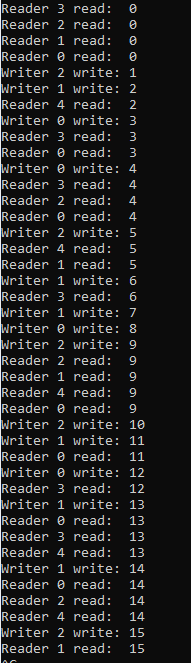
\includegraphics[scale=0.7]{img/read-write-01.png}
	\caption{Демонстрация работы программы.}
	\label{fig:task01}
\end{figure}

\section{Листинги кода}

В листинге \ref{main} представлен исходный код реализующий монитор Хоара <<Читатели-писатели>> для Windows.

\begin{lstlisting}[label=main,caption=Главный файл программы,language=C]
#include <windows.h>
#include <stdio.h>
#include <stdlib.h>

#define OK 0
#define FALSE 0
#define TRUE 1

#define READERS_CNT 5
#define WRITERS_CNT 3

#define WITER_CNT 8
#define RITER_CNT 7

#define WRITE_TIMEOUT 300
#define READ_TIMEOUT 300
#define DIFF 4000

#define CREATE_MUTEX_FAILED 1
#define CREATE_EVENT_FAILED 2
#define CREATE_THREAD_FAILED 3

HANDLE mutex;
HANDLE can_read;
HANDLE can_write;

LONG active_readers = 0;
LONG waiting_writers = 0;
LONG waiting_readers = 0;

int active_writer = FALSE;
int value = 0;

void start_read(void) {
	InterlockedIncrement(&waiting_readers);

	if (active_writer || (WaitForSingleObject(can_write, 0) == WAIT_OBJECT_0 && waiting_writers))
	{
		WaitForSingleObject(can_read, INFINITE);
	}

	WaitForSingleObject(mutex, INFINITE);
	InterlockedDecrement(&waiting_readers);
	InterlockedIncrement(&active_readers);
	
	SetEvent(can_read);
	ReleaseMutex(mutex);
}


void stop_read(void) {
	InterlockedDecrement(&active_readers);
	if (active_readers == 0) {
		ResetEvent(can_read);
		SetEvent(can_write);
	}
}

DWORD WINAPI run_reader(CONST LPVOID lpParams) {
	srand(time(NULL) + WRITERS_CNT);
	int sleep_time;

	for (size_t i = 0; i < RITER_CNT; i++) {
		sleep_time = READ_TIMEOUT + rand() % DIFF;
		Sleep(sleep_time);
		start_read();
		printf("Reader %d read:  %d\n", (int)lpParams;, value);
		stop_read();
	}

	return OK;
}


void start_write(void) {
	InterlockedIncrement(&waiting_writers);
	
	if (active_writer || active_readers > 0) {
		WaitForSingleObject(can_write, INFINITE);
	}
	
	InterlockedDecrement(&waiting_writers);
	active_writer = TRUE;
}


void stop_write(void) {
	active_writer = FALSE;
	
	if (waiting_readers) {
		SetEvent(can_read);
	} else {
		SetEvent(can_write);
	}
}

DWORD WINAPI run_writer(CONST LPVOID lpParams) {
	srand(time(NULL)+ READERS_CNT);
	int sleep_time;
	
	for (int i = 0; i < WITER_CNT; ++i) {
		sleep_time = WRITE_TIMEOUT + rand() % DIFF;
		Sleep(sleep_time);
		start_write();

		printf("Writer %d write: %d\n", (int)lpParams;, ++value);
		stop_write();
	}
	
	return OK;
}

int main(void) {
	HANDLE writers_threads[WRITERS_CNT];
	HANDLE readers_threads[READERS_CNT];

	if (!(mutex = CreateMutex(NULL, FALSE, NULL))) {
		perror("Failed call of CreateMutex");
		return CREATE_MUTEX_FAILED;
	}

	if (!(can_read = CreateEvent(NULL, FALSE, FALSE, NULL)) || !(can_write = CreateEvent(NULL, FALSE, FALSE, NULL))) {
		perror("Failed call of CreateEvent");
		return CREATE_EVENT_FAILED;
	}

	for (int i = 0; i < READERS_CNT; ++i) {
		if (!(readers_threads[i] = CreateThread(NULL, 0, run_reader, (LPVOID)i, 0, NULL))) {
			perror("Failed call of CreateThread");
			return CREATE_THREAD_FAILED;
		}
	}

	for (int i = 0; i < WRITERS_CNT; i++) {
		if (!(writers_threads[i] = CreateThread(NULL, 0, run_writer, (LPVOID)i, 0, NULL))) {
			perror("Failed call of CreateThread");
			return CREATE_THREAD_FAILED;
		}
	}

	WaitForMultipleObjects(READERS_CNT, readers_threads, TRUE, INFINITE);
	WaitForMultipleObjects(WRITERS_CNT, writers_threads, TRUE, INFINITE);

	CloseHandle(mutex);
	CloseHandle(can_read);
	CloseHandle(can_write);
	
	return OK;
}
\end{lstlisting}



\bibliographystyle{utf8gost705u}  % стилевой файл для оформления по ГОСТу

\bibliography{51-biblio}          % имя библиографической базы (bib-файла)


\end{document}
